Now that we have a camera and a method for generating camera rays, we can begin rendering scene objects. One of the simplest primitives to draw using a ray tracer is a sphere which can be defined as follows:
$$(\Vec{S} - \Vec{P})^2 = r^2$$
\begin{tcolorbox}
\textbf{Note:} Vector multiplications in the following equations should be treated as dot products returning a scalar value.
\end{tcolorbox}
\noindent
Where $\Vec{S}$ represents a point on the sphere's surface in the form $\begin{bmatrix} x, y, z \end{bmatrix}$, $\Vec{P}$ represents the origin of the sphere in the same form as $\Vec{S}$, and $r$ represents the sphere's radius. Given a sphere and a ray, our goal is to find their point(s) of intersection. Recall our earlier definition of a ray as $\Vec{O} + t\hat{D}$ where $\Vec{O}$ is the ray's origin, $\hat{D}$ is the ray's direction, and $t$ is a distance along $\hat{D}$ from the ray's origin. This can be substituted for $\Vec{S}$ in the sphere definition to get the following:
$$(\Vec{O} + t\hat{D} - \Vec{P})^2 = r^2$$
Solving for $t$ in the above equation will yield the distance(s) along the ray where it intersects the sphere.
\begin{align*}
    &\Vec{O}^2 + \Vec{O}t\hat{D} - \Vec{O}\Vec{P} + \Vec{O}t\hat{D}  + t^2\hat{D}^2 - t\hat{D}\Vec{P} - \Vec{O}\Vec{P} - \Vec{P}t\hat{D} + \Vec{P}^2 = r^2 &\text{expand left side}&\\
    &\Vec{O}^2 + \Vec{P}^2 - 2\Vec{O}\Vec{P}  - r^2 + 2\Vec{O}\hat{D}t - 2\hat{D}\Vec{P}t + \hat{D}^2t^2 = 0 &\text{combine terms and move $r^2$}&\\
    &\hat{D}^2t^2 + (2\Vec{O}\hat{D}-2\hat{D}\Vec{P})t + \Vec{O}^2 + \Vec{P}^2 - 2\Vec{O}\Vec{P} - r^2 = 0 &\text{rearrange terms}&
\end{align*}
Notice that the equation above is a quadratic in the form $at^2 + bt + c = 0$ where 
\begin{align*}
    a &= \hat{D}^2 &&= 1 \\
    b &= 2\Vec{O}\hat{D}-2\hat{D}\Vec{P} &&= 2\hat{D}(\Vec{O}-\Vec{P}) \\
    c &= \Vec{O}^2 + \Vec{P}^2 - 2\Vec{O}\Vec{P} - r^2 &&= (\Vec{O}-\Vec{P})^2-r^2
\end{align*}
Therefore, we can attempt solving using the quadratic formula:
$$
t = \frac{-2\hat{D}(\Vec{O}-\Vec{P}) \pm \sqrt{(2\hat{D}(\Vec{O}-\Vec{P}))^2 - 4((\Vec{O}-\Vec{P})^2-r^2)}}{2}
$$
Like with any other quadratic, we can use the discriminant, in this case $d = (2\hat{D}(\Vec{O}-\Vec{P}))^2 - 4((\Vec{O}-\Vec{P})^2-r^2)$, to make conclusions about the number of solutions:
\begin{enumerate}
    \item $d < 0$: There are no intersection points between the ray and the sphere
    \item $d = 0$: There is exactly one intersection point between the ray and the sphere
    \item $d > 0$: There are exactly 2 intersection points between the ray and the sphere
\end{enumerate}
If we have at least one solution, we can obtain more information based on the value(s) of $t$:
\begin{enumerate}
    \item $t < 0$: The intersection point is behind the camera and is not visible
    \item $t \geq 0$: The intersection point is at or in front of the camera's position and is visible
\end{enumerate}
For now, to quickly visualize the sphere, we will fill pixels whose corresponding camera ray's have intersection(s) with the sphere at $t \geq 0$ with a solid green color. When we have two points of intersection, we will only use the one with a lower $t$ in order to only render the camera facing part of the sphere while ignoring the back. Placing a sphere at the point $\begin{bmatrix} 0, 0, 1 \end{bmatrix}$ with radius $r = 1$ and a camera at $\begin{bmatrix} 0, 0, -1 \end{bmatrix}$ with direction $\begin{bmatrix} 0, 0, 1 \end{bmatrix}$ and the same viewport dimensions as earlier, we get the following image:

\begin{figure}[H]
    \centering
    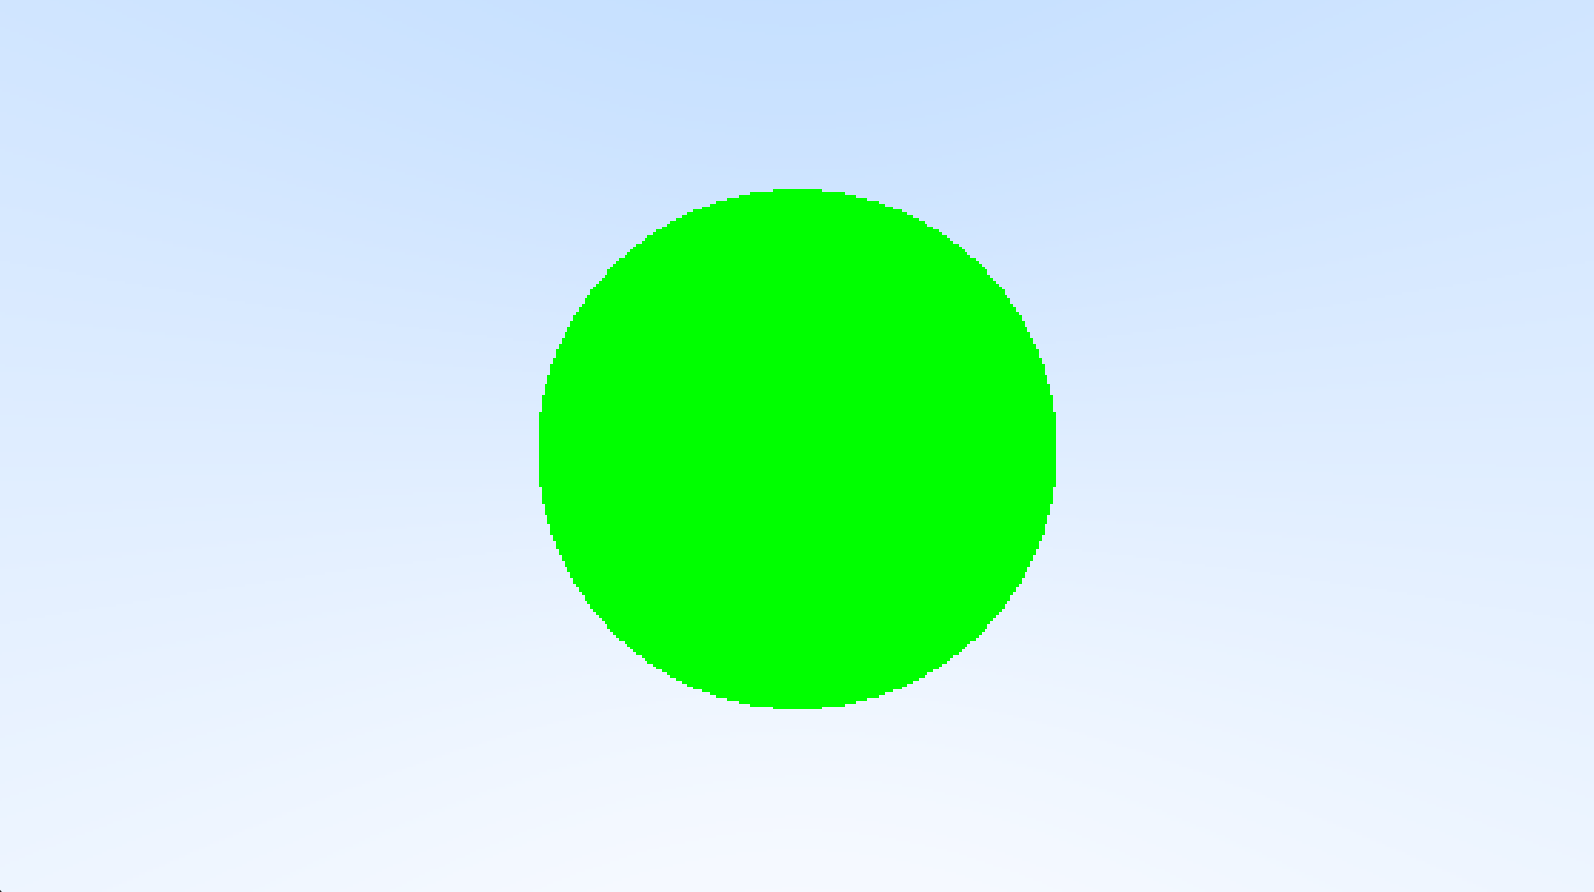
\includegraphics[scale=0.5]{figures/GreenSphere.png}
    \caption{Sphere rendered without shading}
    \label{fig:green_sphere}
\end{figure}
\noindent
Of course, the rendered image above looks more like a circle than a sphere because we have yet to introduce lighting and shading. A key piece of information we need for lighting calculations is the sphere's normal at a point on its surface. The surface normal, $\hat{N}$, can be thought of as a normalized three dimensional vector that is perpendicular to the sphere's surface. 
\begin{figure}[H]
    \centering
    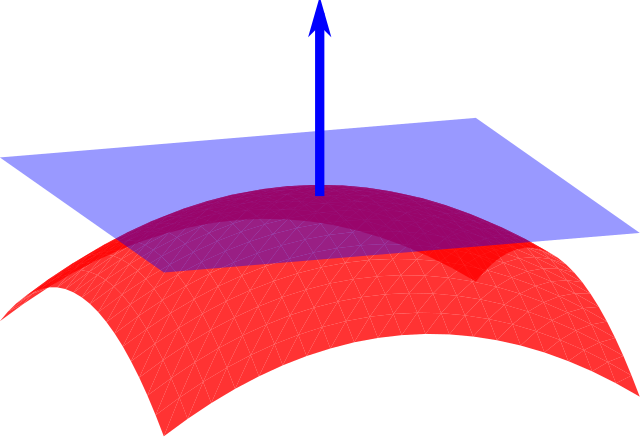
\includegraphics[scale=0.3]{figures/normal.png}
    \caption{Illustration of a surface normal (blue arrow) (Wikimedia Commons)}
    \label{fig:normal_example}
\end{figure}
\noindent
Given a point of intersection $\Vec{I}$ and the center of the sphere $\Vec{P}$, we can calculate the normal as follows:
$$\hat{N} = \frac{\Vec{I} - \Vec{P}}{|\Vec{I} - \Vec{P}|}$$
\begin{tcolorbox}
\textbf{Note:} Given that we have solved for $t$, finding the point of intersection simply involves substituting the value of $t$ into the definition of a ray $\Vec{O} + t\hat{D}$.
\end{tcolorbox}
\noindent
To visualize this, we can assign colors based on the surface normal at each intersection point with the following mapping:
$$\text{Color} = \frac{\hat{N} + \begin{bmatrix} 1\\ 1\\ 1 \end{bmatrix}}{2}$$
This yields the following image of our earlier sphere:
\begin{figure}[H]
    \centering
    
\includegraphics[scale=0.5]{figures/SphereNormal.png}
    \caption{Sphere visualized with surface normals}
    \label{fig:sphere_normal}
\end{figure}